\documentclass[addpoints,spanish, 12pt,a4paper,cancelspace]{./include/gexam}

 %%%%%%%%%%%%%%%%%%%%%%%%%%%
 \renewcommand{\documentName} { Sistema de coordenadas cartesianos }
 \renewcommand{\documentContent} { \phantom{ } } 
 \renewcommand{\waterMark} { Modelo 5 } 

 % Configuración del documento.
 \renewcommand{\schoolSubject} { Examen Matemáticas 2º ESO  }
\renewcommand{\school} { IES José de Churriguera  }
\renewcommand{\academicPeriod} { Curso 2022/2023 }

\renewcommand{\autor} { Andrés Giménez Muñoz }
\renewcommand{\emailAuthor} { andresprofemates@outlook.es }
\renewcommand{\autorSing}{ Profesor: Andrés } 
 %%%%%%%%%%%%%%%%%%%%%%%%%%%
 
% \renewcommand{\thepartno}{\arabic{partno}}
%  \renewcommand{\thepartno}{\thecurrentpartno.\arabic{partno}}

% \renewcommand{\partlabel}{$$$(\thequestion.\arabic{partno}$$(}
% \renewcommand{\subpartlabel}{$$$(\thepart.\arabic{subpartno}$$(}

\renewcommand\subpartlabel{\thesubpart}
\renewcommand\subpartshook{\renewcommand\makelabel[1]{##1\hfil }} 
 
 %%%%%%%%%%%%%%%%%%%%%%%%%%%
 % Exam configuration
 %\pointsdroppedatright   %% No mostrar la puntuación
 \pointsinrightmargin{} % Para poner las puntuaciones a la derecha. Se puede cambiar. Si se comenta, sale a la izquierda.
 \extrawidth{-1.5cm} %Un poquito más de margen por si ponemos textos largos.
 \marginpointname{ \emph{\points}}
 
 %% Si se comenta no aparecerán los espacios de la solución.
 %\nocancelspace
 
 %% Puntuación a la izquierda.
%  \nopointsinrightmargin 

 %% Esto es de la clase exam. Si dejamos sin comentar \printanswers, se mostraran las soluciones. 
 %% Si la comentamos y dejamos sin comentar \noprintanswers, pues no se muestran las soluciones.
 % \printanswers
 %\noprintanswers
 
 %%%%%%%%%%%%%%%%%%%%%%%%%%%
 
 \begin{document}
 
%  \StudentData{}
%  \GradeTableHeader{}
 
 \justifying

% \begin{center}
%     \fbox{\fbox{\parbox{6.5in}{             
%                 \begin{itemize}
%                     \item Deben aparecer todas las operaciones, no vale solo con indicar el resultado.
%                     \item Se podrán quitar hasta cinco décimas por falta de claridad o rigor en el desarrollo de las respuestas o por una mala presentación.
%                     \item Se valorará que se indiquen las cuentas en línea, realizando las operaciones en el margen.
%                     \item No se puede utilizar la calculadora.
%                 \end{itemize}
%             }}}
% \end{center}
 
 \begin{questions}
    
    %% Gato
    \question Dibuja los puntos en el orden en el que aparece y únelos con segmentos de línea. \\
    \small
    Trazo 1:
    $(2, -3)$ $(-2, -3)$ $(-4, -1)$ $(-5, 1)$ $(-6, 5)$ $(-6, 15)$ $(-5, 17)$ $(-3, 18)$ $(3, 18)$ $(5, 17)$ $(6, 15)$ $(6, 5)$ $(5, 1)$ $(4, -1)$ $(2, -3)$

    Trazo 2: $(-4, -1)$ $(-4, 3)$ $(-6, 6)$ $(-5, 9)$ $(-5, 15)$ $(-3, 16)$ $(-2, 16)$ $(-1, 11)$ $(1, 11)$ $(2, 16)$ $(3, 16)$ $(5, 15)$ $(5, 9)$ $(6, 6)$ $(4, 3)$ $(4, -1)$

    Trazo 3: $(-4,1)$ $(-3, 0)$ $(-2, 1)$ $(2, 1)$ $(3, 0)$ $(4, 1)$

    Trazo 4: $(-4, 8)$ $(-1, 7)$ $(1, 7)$ $(4, 8)$ $(5, 7)$ $(4, 6)$ $(2, 6)$ $(1, 7)$ $(-1, 7)$ $(-2, 6)$ $(-4, 6)$ $(-5, 7)$ $(-4, 8)$

    Trazo 5: $(-6, 5)$ $(-9, 5)$ $(-11, 4)$ $(-11, 3)$ $(-15, 3)$ $(-20, 1)$ Trazo 6: $(6, 5)$ $(9, 5)$ $(11, 4)$ $(11, 3)$ $(16, 3)$ $(20, 1)$

    Trazo 7: $(-13, -20)$ $(-14, -16)$ $(-13, -13)$ $(-14, -10)$ $(-15, -13)$ $(-16, -17)$ $(-18, -20)$ 

    Trazo 8: $(13, -20)$ $(14, -16)$ $(13, -13)$ $(14, -10)$ $(15, -13)$ $(16, -17)$ $(18, -20)$ 

    Trazo 9: $(-13, -11)$ $(-12, -10)$ $(-12, -8)$ $(-11, -8)$ $(-10, -6)$ $(-8, -6)$ $(-2, -9)$ $(2, -9)$ $(8, -6)$ $(10, -6)$ $(11, -8)$ $(12, -8)$ $(12, -10)$ $(13, -11)$

    Trazo 10: $(-2, -14)$ $(-1, -13)$ $(1, -13)$ $(2, -14)$ $(2, -17)$ $(1, -18)$ $(-1, -18)$ $(-2, -17)$ $(-2, -14)$ 

    Trazo 11: $(6, 4)$ $(7, 1)$ $(6, -5)$ $(8, -2)$ $(10, -3)$ $(11, -5)$ $(11, -6)$ $(12, -6)$ $(14, -3)$ $(17, -3)$ $(20, -4)$ $(17,-3)$ $(14, -3)$ $(14, 1)$ $(13, 3)$

    Trazo 12: $(-6, 4)$$(-7, 1)$$(-6, -5)$$(-8, -2)$$(-10, -3)$$(-11, -5)$$(-11, -6)$$(-12, -6)$ $(-14, -3)$ $(-17, -3)$ $(-20, -4)$ $(-17,-3)$$(-14, -3)$ $(-14, 1)$ $(-13, 3)$

    Trazo 13: $(5,-13)$ $(6,-14)$ $(6,-17)$ $(3, -20)$ $(2,-19)$ $(-2,-19)$ $(-2, -19)$ $(-4, -17)$ $(-4, -14)$ $(-2, -12)$ $(2,-12)$ $(4, -9)$ $(8, -8)$ $(11, -8)$

    Trazo 14: $(-5,-13)$ $(-6,-14)$ $(-6,-17)$ $(-3, -20)$ $(-2,-19)$ $(2,-19)$ $(2, -19)$ $(4, -17)$ $(4, -14)$ $(2, -12)$ $(-2,-12)$ $(-4, -9)$ $(-8, -8)$ $(-11, -8)$

    Trazo 15: $(-5,-4)$ $(-2,-5)$ $(-1,-6)$ $(1,-6)$ $(2,-5)$ $(5,-4)$

    \normalsize

    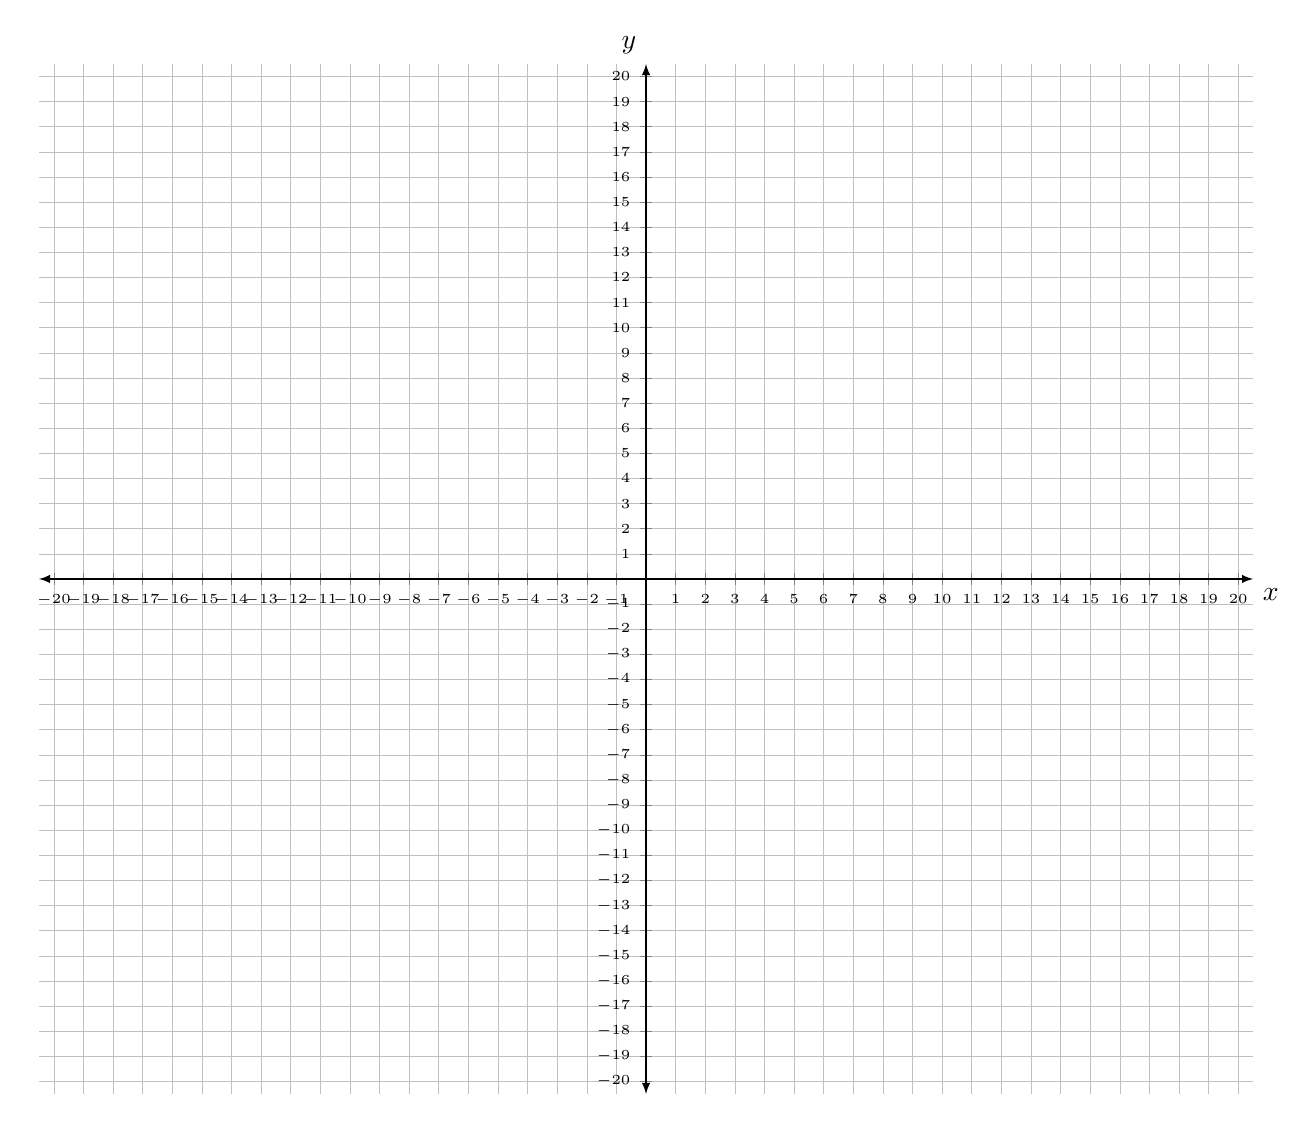
\begin{tikzpicture}[scale=1]
        \begin{axis}[
            axis x line=center,
            axis y line=center,
            xlabel = {$x$},
            ylabel = {$y$},
            xmin=-20,xmax=20,
            ymin=-20,ymax=20,
            xtick distance=1, 
            ytick distance=1, 
            grid=both,
            grid style={line width=.1pt, draw=gray!10},
            major grid style={line width=.2pt,draw=gray!50},
            axis lines=middle,
            axis line style={<->},
            minor tick num=0,
            enlargelimits={abs=0.5},
            axis line style={latex-latex},
            ticklabel style={font=\tiny},
            % ticklabel style={font=\tiny,fill=white},
            % xlabel style={at={(ticklabel* cs:1)},anchor=north west},
            % ylabel style={at={(ticklabel* cs:1$)},anchor=south west},
            xlabel style={below right},
            ylabel style={above left},
            width=17cm,
        ]
        
        \end{axis}

    \end{tikzpicture}

\end{questions}
 
\end{document}